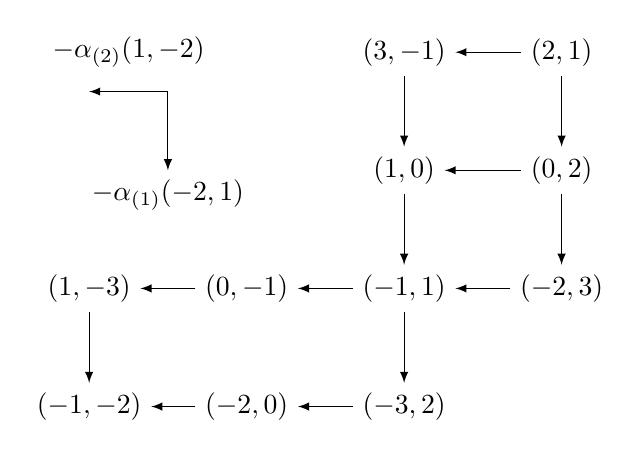
\begin{tikzpicture}

\node (v1) at (-4,-4.5) {$(2,1)$};
\node (v2) at (-4,-6) {$(0,2)$};
\node (v3) at (-4,-7.5) {$(-2,3)$};
\node (v4) at (-6,-4.5) {$(3,-1)$};
\draw [-latex] (v1) edge (v2);
\draw [-latex] (v2) edge (v3);
\draw [-latex] (v1) edge (v4);
\node (v5) at (-6,-6) {$(1,0)$};
\node (v6) at (-6,-7.5) {$(-1,1)$};
\node (v7) at (-6,-9) {$(-3,2)$};
\draw [-latex] (v4) edge (v5);
\draw [-latex] (v5) edge (v6);
\draw [-latex] (v6) edge (v7);
\draw [-latex] (v2) edge (v5);
\node (v8) at (-8,-7.5) {$(0,-1)$};
\node (v9) at (-10,-7.5) {$(1,-3)$};
\node (v10) at (-8,-9) {$(-2,0)$};
\node (v11) at (-10,-9) {$(-1,-2)$};
\draw [-latex] (v6) edge (v8);
\draw [-latex] (v8) edge (v9);
\draw [-latex] (v7) edge (v10);
\draw [-latex] (v10) edge (v11);
\draw [-latex] (v3) edge (v6);
\draw [-latex] (v9) edge (v11);


\draw [-latex] (-9,-5) -- (-9,-6);
\draw [-latex] (-9,-5) -- (-10,-5);
\node [below] at (-9,-6) {$ -\alpha_{(1)} \rightsquigarrow (-2,1)$};
\node at (-9.5,-4.5) {$-\alpha_{(2)} \rightsquigarrow (1,-2)$};

\end{tikzpicture}